\documentclass{article}
\usepackage{geometry}
\usepackage{graphicx}
\usepackage{enumitem}
\usepackage{anyfontsize}
\usepackage{setspace}
\usepackage{microtype}
\usepackage{multicol}
\usepackage[russian]{babel}
\usepackage{float}
\geometry{
  left=2.1cm,
  right=2.1cm, 
  top=1.8cm,
  bottom=1.8cm
}

\begin{document}

\begin{multicols}{2}

\raggedright

\setstretch{1.5}

\begin{minipage}[t]{0.49\textwidth} \fontsize{9}{7}\selectfont
way to increase the accuracy. The model is implemented on the basis of the IoT platform for building a subsystem of IT diagnostics of patients as part of the smart city project using elements of OSTIS technology [14].

\begin{center}
\textsc{V. C\resizebox{!}{1.3ex}{ONCLUSION}}
\end{center}

\hspace{0.2cm}  The aim of this paper was to explore the performance of GRU neural networks in voice recognition tasks within neurological diseases. We used a 6-layer GRU model that was trained and tested on the Parkinson’s public voice dataset and the Alzheimer’s public voice dataset. With the experimental results, we found that.

\begin{enumerate}[label=\arabic*), noitemsep]
  \item On the Parkinson’s public voice dataset, our model can achieve 86.66\% accuracy, which has better performance than traditional machine learning methods. However, the accuracy on the Alzheimer public voice dataset was only 68.27\%, indicating that the 6-layer GRU model does not have good generalization ability.
  \item During the training of the model, we noticed that the training error of the model was gradually decreasing with the increase of training times, but the testing error started to increase. This indicated that the model appeared overfitting phenomenon.
  \item We also explored our scheme to implement the GRU model on the IoT. The scheme has potential for practical applications and provides a reference for research in related fields.
\end{enumerate}
\hspace{0.2cm}Summing up, our experimental results showed that the GRU model can be deployed on IoT platforms to solve part of the problem of IT diagnostics of neurological disorders by recognizing changes in patients’ speech.

\begin{center}
\textsc{R\resizebox{!}{1.3ex}{EFERENCES}}
\end{center}

\begin{enumerate}[label={[\arabic*]}, noitemsep]

{\fontsize{8}{7}\selectfont \item B. Lu, B. Li, H. Chang, Z. Li, L. Chen, N. Zhu, Z. Zhou, H. Li, X. Wang, Y. Cui \textit{et al.}, ``A practical alzheimer disease classifier via brain imaging-based deep learning on 85,721 samples [preprint],'' \textit{Neuroscience}, 2020}.

{\fontsize{8}{7}\selectfont \item D. Mukherji, M. Mukherji, and N. Mukherji,``Early detection of alzheimer's disease using neuropsychological tests: a predict-diagnose approach using neural networks,'' \textit{Brain Informatics}, vol. 9, no. 1, pp. 1-26, 2022}.

{\fontsize{8}{7}\selectfont \item D. Payares-Garcia, J. Mateu, and W. Schick, ``Spatially informed bayesian neural network for neurodegenerative diseases classification,'' \textit{Statistics in medicine}, vol. 42, no. 2, pp. 105-121, 2023}.

{\fontsize{8}{7}\selectfont \item A. Sheikhtaheri and F. Sabermahani, ``Applications and outcomes of internet of things for patients with alzheimer's disease/dementia: A scoping review,'' \textit{BioMed Research International}, vol. 2022, 2022}.

{\fontsize{8}{7}\selectfont \item S. Saba Raoof, M. Durai et al., ``A comprehensive review on smart health care: Applications, paradigms, and challenges with case studies,'' \textit{Contrast Media \& Molecular Imaging}, vol. 2022, 2022.}

{\fontsize{8}{7}\selectfont \item R. R. Irshad, A. A. Alattab, O. A. S. Alsaiari, S. S. Sohail, A. Aziz, D. i. Madsen, and K. M. Alalayah, ``An optimization-linked intelligent security algorithm for smart healthcare organizations,'' in \textit{Healthcare}, vol. 11, no. 4. MDPI, 2023, p. 580.}

{\fontsize{8}{7}\selectfont \item R. A. Bernardes, F. Ventura, H. Neves, M. I. Fernandes, and P. Sousa, ``Wearable walking assistant for freezing of gait with environmental iot monitoring: A contribution to the discussion,'' \textit{Frontiers in Public Health}, vol. 10, 2022.}
\end{enumerate}

\end{minipage}

\raggedleft
\begin{minipage}[t]{0.48\textwidth}

\setstretch{0.8}

\begin{enumerate}[label={[\arabic*]}, start=8, noitemsep]
{\fontsize{8}{7}\selectfont \item  F. L. Darley, A. E. Aronson, and J. R. Brown, ``Differential diagnostic patterns of dysarthria," \textit{Journal of speech and hearing research}, vol. 12, no. 2, pp. 246--269, 1969.}

{\fontsize{8}{7}\selectfont \item B. E. Sakar, M. E. Isenkul, C. O. Sakar, A. Sertbas, F. Gurgen, S. Delil, H. Apaydin, and O. Kursun, ``Collection and analysis of a parkinson speech dataset with multiple types of sound recordings," \textit{IEEE Journal of Biomedical and Health Informatics}, vol. 17, no. 4, pp. 828--834, 2013.}

{\fontsize{8}{7}\selectfont \item F. Eyben, K. R. Scherer, B. W. Schuller, J. Sundberg, E. André, C. Busso, L. Y. Devillers, J. Epps, P. Laukka, S. S. Narayanan \textit{et al.}, ``The geneva minimalistic acoustic parameter set (gemaps) for voice research and affective computing," \textit{IEEE transactions on affective computing}, vol. 7, no. 2, pp. 190--202, 2015.}

{\fontsize{8}{7}\selectfont \item C. O. Sakar, G. Serbes, A. Gunduz, H. C. Tunc, H. Nizam, B. E. Sakar, M. Tutuncu, T. Aydin, M. E. Isenkul, and H. Apaydin, ``A comparative analysis of speech signal processing algorithms for parkinson's disease classification and the use of the tunable q-factor wavelet transform," \textit{Applied Soft Computing}, vol. 74, pp. 255--263, 2019.}

{\fontsize{8}{7}\selectfont \item A. M. Lanzi, A. K. Saylor, D. Fromm, H. Liu, B. MacWhinney, and M. L. Cohen, ``Dementiabank: Theoretical rationale, protocol, and illustrative analyses," \textit{American Journal of Speech-Language Pathology}, pp. 1--13, 2023.}

{\fontsize{8}{7}\selectfont \item A. Luque, A. Carrasco, A. Martín, and A. de Las Heras, ``The impact of class imbalance in classification performance metrics based on the binary confusion matrix," \textit{Pattern Recognition}, vol. 91, pp. 216--231, 2019.}

{\fontsize{8}{7}\selectfont \item D. Shunkevich, ``Agent-oriented problem solvers of intelligent systems component," autoref. of PhD thesis in tech. sciences: 05.13.17 / Belarusian State University of Informatics and Radioelectronics, Minsk, pp. 1--24, 2018.}
\end{enumerate}

\begin{center}
\textbf{\fontsize{12}{7}\selectfont Технология распознавания нейрологических заболеваний с использованием нейронной сети закрытого рекуррентного блока и интернета вещей}
\end{center}

\begin{center}
\fontsize{12}{7}\selectfont Вишняков В. А., Ивей С., Чуюэ Ю.
\end{center}

\setstretch{1.3}
\hspace{0.2cm} \fontsize{8}{7}\selectfont В этой статье авторы предложили метод распознавания неврологических заболеваний с использованием закрытой рекуррентной нейронной сети и поддержки Интернета вещей (IoT), который был проверен на примере болезни Альцгеймера (БА) и болезни Паркинсона (БП). В этом методе сначала предварительно выделяются и ослабляются голосовые данные, затем голосовые сигналы сегментируются с помощью скользящего фиксированного окна с использованием функции окна Хэмминга. Затем извлекаются голосовые характеристики eGeMAPSv02 из сигнала окна, вводятся эти характеристики в модель нейронной сети с закрытым рекуррентным модулем для ее обучения, тестирования и достижения диагноза заболевания. Результаты исследования показали, что, несмотря на ограниченную способность модели gated recurrent unit к обобщению, она может эффективно обеспечивать распознавание голоса при выявлении части неврологических заболеваний. Модель реализуется на базе платформы IoT для построения подсистемы ИТ-диагностики пациентов а рамках проекта умного города. Код хранится \url{https://github.com/HkThinker/Technology-of-neural-disease-recognition}.

\hspace{0.2cm}Ключевые слова— нейронная сеть с закрытым рекуррентным модулем, сеть Интернета вещей, распознавание голоса, неврологические заболевания.

\hspace{0.2cm}Термины индекса — закрытая рекуррентная нейронная сеть, Интернет вещей, распознавание голоса, неврологические заболевания.

\begin{flushright}
Received 12.03.2023
\end{flushright}

\setcounter{page}{246}

\end{minipage}
\end{multicols}

\begin{newpage}
\begin{center}
\fontsize{20}{7}\selectfont \textbf{Hand Gesture Recognition Based on Skeletal Image Properties}

\vspace{0.1cm}\fontsize{12}{7}\selectfont J. Ma and V. Yu. Tsviatkou and A. A. Boriskevich

\vspace{0.1cm} \textit{Belarusian State University of Informatics and Radioelectronics}

Minsk, Belarus

\fontsize{11}{7}\selectfont Email: majun1313@hotmail.com, vtsvet@bsuir.by, anbor@bsuir.by
\end{center}
\end{newpage}

\begin{multicols}{2}

\raggedright
\begin{minipage}[t]{0.47\textwidth}

\setstretch{1.3}
\vspace{1.3cm} \hspace{0.2cm} \fontsize{8}{7}\selectfont \textbf{\textit{Abstract}—Hand gesture Recognition is an important task and can be used in a lot of applications. In intelligen systems, hand gesture recognition can be used to access information through a video interface. In recent years, skeleton-based hand gesture recognition become a popular research topic. The existing methods have the low discriminative power due to sensitivity of features to image noise. We have proposed new methods to decrease the influence of the noise to extract hand image features. The objective of the research is to improve the hand gesture classification accuracy. A hand gesture recognition method based on skeleton image properties is developed. For 5 classes recognition, this approach allows us to increase the classification accuracy on test set from 0.4\% till 20.4\% as compared with existing well-known methods.For 10 classes recognition, this approach allows us to increase the classification accuracy from 5\% till 18\% as compared wit existing well-known methods.}

\hspace{0.2cm} \textbf{\textit{Keywords}—Color images, Skeleton images, hand gesture feature, Machine Learning, Classification Accuracy.}

\begin{center}
\fontsize{9}{7}\selectfont \textsc{I. I\resizebox{!}{1.3ex}{NTRODUCTION}}
\end{center}

\setstretch{1.7}

\fontsize{10}{7}\selectfont \hspace{0.2cm}Hand gesture recognition is widely used in many applications such as sign language recognition [1], clinical and health [2], and robot control [3]. Open semantic technologies provide the ability to access the knowledge base of an intelligent system using a video interface. The inclusion of a hand gesture recognition system in the video interface makes it easier to enter commands and data into an intelligent system.

\hspace{0.2cm}There are two existing practical approaches to recognizing hand gestures [4]. The first approach is based on data gloves (wearable or direct contact) [5,6], and the second is based on computer vision, which does not require special sensors except cameras [7]. Moreover, vision-based methods can provide contactless communication between humans and computers, making them suitable for ordinary use.

\hspace{0.2cm}As one of the types of camera vision-based approaches [4], skeleton-based approaches are attracting much attention in recent years since the skeleton feature describes geometric attributes and constraints and easily translates features and data correlations [8]. The skeleton-based approaches can further be classified as RGB-based [9] and RGB-D-based [10]- [12] approaches according to the different ways of obtaining the skeletal images. The

\end {minipage}

\raggedleft
\begin{minipage}[t]{0.48\textwidth}
\vspace*{1.25cm}
\setstretch{0.93}
RGB-D-based approaches adopt the depth sensor of the Kinect camera to obtain the skeletal image. One of the merits of these methods is that the lighting, shade, and color did not affect the obtained skeletal image. However, the depth camera’s cost, size, and availability will limi their use. On the contrary, RGB-based approaches only require standard cameras. However, it must first conver the RGB images into grayscale images and then follow binarization and skeletonization to extract the skeletons. The skeletons extracted by this kind of method may include many useless skeletal branches or skeletal rings that are caused by the noise. The noise problem will b evident when the contrast of the input image is low. Since the existence of the noise, the accuracy of hand gesture recognition using RGB skeleton-based approaches are not satisfying. However, it would be a promising method if the effect of the noise could be reduced. 

\hspace{0.2cm}In the past several decades, many denoise methods have been proposed to alleviate the effects of noise on the skeletonization algorithm and produce stable skeletons as much as possible. These methods can be concluded into three different types, which are skeletonizationbased denoising approaches [13]- [16], pruning-based denoising approaches [17]- [19], and scale-space-based denoising approaches [20], [21].

\hspace{0.2cm}In this paper, a hand gesture recognition system based on skeleton image properties is developed, in which skeleton images are extracted by using different combinations of the skeletonization and denoising method. The objective of the research is to improve hand gesture classification accuracy.

\begin{center}
\fontsize{9}{7}\selectfont \textsc{II. I\resizebox{!}{1.3ex}{ELATED}} \textsc{M\resizebox{!}{1.3ex}{ETHODS}}
\end{center}

\hspace{0.2cm}In this section, some skeletonization and denoising methods used in our hand gesture recognition system are introduced. There are five skeletonization methods implemented, two of which are classical skeletonization methods, and others proposed by us. In addition, a postpruning method and a space-based denoising approach are also deployed in this system.

\begin{flushleft}
\textit{A. Image Skeletonization Method}
\end{flushleft}

\hspace{0.2cm}OPTA algorithm [22] is a classical parallel skeletonization method proposed by Roland T. Chin et al. This

\end {minipage}
\end{multicols}

\begin{newpage}

\renewcommand{\figurename}{Figure}
\begin{figure}[H]
    \centering
    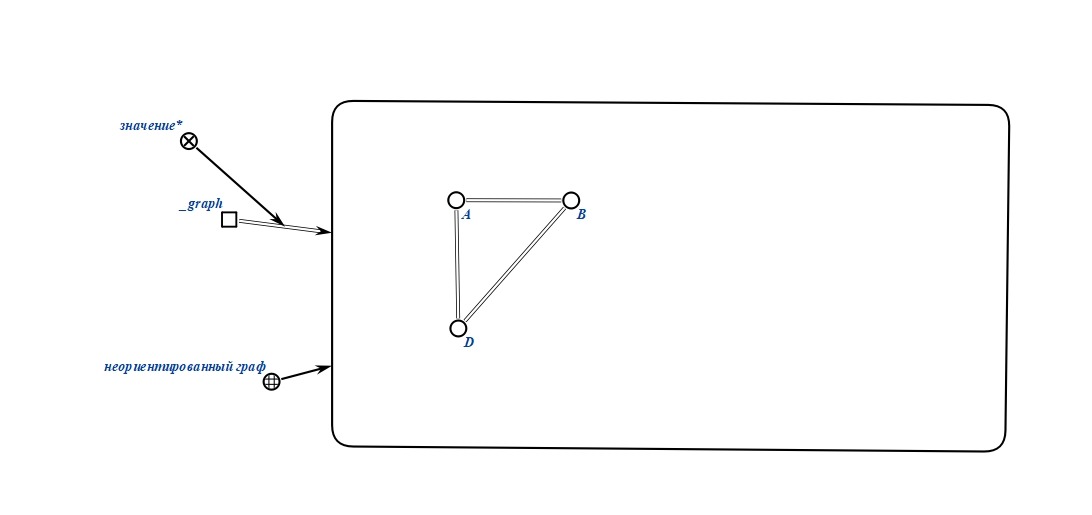
\includegraphics[width=0.5\linewidth]{image.png}
     \caption {General block-scheme of the hand gesture reognition.}
    \label{fig:enter-label}
\end{figure}

\begin{multicols}{2}

\raggedright
\begin{minipage}[t]{0.47\textwidth}

algorithm uses eight 3 × 3 thinning templates to remove the pixels. In addition, two other restoring templates are applied to address the breakage and disappearance of horizontal and vertical limbs with double-pixel widths. The drawback of this algorithm is that it is susceptible to noise. ZS algorithm [23] is another classical parallel skeletonization method, which is one of the most popular methods since it can offset the influence of the noise to some extent by breaking one iteration in OPCA into two sub-iterations. Therefore, the computation speed of the 

\hspace{0.2cm}ZS method is slower than OPTA. In addition, the ZS algorithm has some potential problems, such as sometimes it may suffer the problem of excessive erosion, and it fails to maintain one-pixel width, which may increase the difficulty when applied to recognition tasks. 

\hspace{0.2cm}Based on these two classical methods, we have proposed three new skeletonization methods: OPCA, ZSM, and OPTA. 

\hspace{0.2cm}OPCA [24] is a denoising version of the OPTA algorithm by modifying some deletion conditions. It is more robust than the OPTA method and, at the same time, shares a similar computation speed with the OPTA method. In addition, it can achieve a single-pixel width. However, it is more sensitive to the noise than the ZS algorithm. 

\hspace{0.2cm}ZSM [25] is an improved version of the ZS algorithm, in which the drawbacks of excessive erosion are overcomed and it can achieve single pixel width by adopting extra five thinning templates. The denoise ability of this algorithm is similar to the ZS algorithm. However, this method is still a sub-iterative method as the ZS algorithm.

\end {minipage}

\raggedleft
\begin{minipage}[t]{0.48\textwidth}

MOPCA [26] is the improved version of the OPCA, in which there is a total of 13 templates are used to enhance the robustness of the algorithm to the noise. This method combines the merits of ZS algorithms and OPTA algorithms. It is insensitive to noise as the ZS and as fast as the OPTA method. 

\vspace{0.4cm} \textit{B. Post-pruning and Scale-Space based Denoiseing Method}

\vspace{0.2cm} \hspace{0.2cm}Using denoise-skeletonization can only partly offset the influence of the noise. Therefore, it is necessary to use other denoising techniques to further improve the noise-against ability. As a result, we also proposed a new post-pruning method and a new scale-space denoisin method. 

\hspace{0.2cm}The post-pruning method proposed by us is named DCEM [27], modified from the famous pruning algorithm of DCE [28]. One of the limitations of the DC is that it requires manual tuning of the parameter of the pruning power’s strength. In DCEM, conducting this tedious work is unnecessary, making it more convenient in many applications. 

\hspace{0.2cm}Our proposed scale-space denoising method is ATFM [29], derived from the ATF [30] method. The core idea of the ATF method is first to extract skeletons from different smoothed images that are filtered by using different scale-space filters to the original image. Then, they used their proposed sensitive measure to evaluate these skeletons, from which the skeleton with the lowest score is considered stable. However, their method sometimes may suffered the problem of the deformation of the skeleton. To overcome this problem, we proposed our ATFM method. In our method, the significant modification on

\end{minipage}

\end{multicols}
    
\end{newpage}

\end{document}

